\documentclass[11pt]{article}

% ---------------------------------------------------------------------------
% Beetle: A Reproducible Hybrid-Retrieval Ablation on Small Public Benchmarks
%
% Tables and figures are sourced from the evaluation outputs:
%   eval/results/  -> regenerate LaTeX tables with `python eval/make_tables.py`
%                     (writes paper/tables/*.tex, \input below)
%   eval/figures/  -> Pareto + per-dataset bar charts, \includegraphics below
% so the paper stays consistent with the actual run.
% ---------------------------------------------------------------------------

\usepackage[margin=1in]{geometry}
\usepackage{graphicx}
\usepackage{booktabs}
\usepackage{amsmath}
\usepackage{hyperref}
\usepackage{xcolor}

\graphicspath{{figures/}{../eval/figures/}}

\title{Beetle: A Reproducible Hybrid-Retrieval Ablation\\
       (BM25 + Dense + SPLADE + RRF + Cross-Encoder)\\
       on Small Public Benchmarks}
\author{Akshit Manocha}
\date{\today}

\begin{document}
\maketitle

\begin{abstract}
Hybrid retrieval --- combining lexical (BM25), dense (bi-encoder), and learned-sparse
(SPLADE) signals, optionally followed by a cross-encoder reranker --- is the
de-facto recipe for first-stage-plus-reranking search. Yet for a small system it
is rarely measured rigorously: which family actually wins on a given corpus, does
fusing them help, and what does the reranker cost? \emph{Beetle} answers these
questions on two small, widely-cited BEIR datasets (SciFact and NFCorpus)
with a fully reproducible harness that runs end-to-end on a single laptop (Apple
M4 Pro, MPS/CPU; no external GPU). We do not propose a new retrieval algorithm.
Instead we (i) fix the single highest-impact correctness bug in the original
system --- a dense index that used Euclidean (L2) distance on un-normalized
embeddings rather than cosine similarity --- and quantify the resulting quality
delta; (ii) include SPLADE in a weighted Reciprocal Rank Fusion that the original
system omitted; (iii) report a clean five-system quality--compute ablation (BM25,
dense, SPLADE, hybrid, hybrid+rerank) whose
baselines match published BEIR numbers; and (iv) document a subtle Apple-Silicon
reproducibility hazard --- \texttt{torch.max} returning wrong values for short,
lightly-padded sequences on \texttt{mps} --- that silently halved SPLADE's score
until diagnosed, with a one-line fix. Every number in this paper is produced by a
versioned, pinned-dependency pipeline, and the eight core correctness properties of
the retrieval and metric code are verified with property-based tests.
\end{abstract}

\section{Introduction}
\label{sec:intro}

A practitioner assembling a search system over a specialized corpus faces a
recurring set of questions. Should they use a classical lexical index (BM25), a
neural dense retriever, a learned-sparse model (SPLADE), or some combination?
Does combining them via rank fusion actually improve quality, or merely add
latency? And is a cross-encoder reranker --- typically 50--100$\times$ slower than
first-stage retrieval --- worth its cost? These questions are usually answered by
folklore rather than measurement, particularly in small portfolio-scale systems
that lack an evaluation harness.

Beetle is an existing hybrid search engine that already contained all three
retrieval families, RRF fusion, and a cross-encoder reranker, but had never been
measured on a public benchmark, and contained a subtle but consequential bug: its
FAISS dense index used \texttt{IndexFlatL2} over embeddings that were never
L2-normalized, so ``nearest'' was Euclidean rather than cosine --- the wrong
geometry for sentence-embedding retrieval. This paper re-scopes Beetle into a
measured, reproducible research artifact.

\paragraph{Contributions.}
\begin{enumerate}
  \item A small, fully reproducible evaluation harness over two BEIR datasets
        (SciFact and NFCorpus) computing nDCG@10, MRR@10, and Recall@100,
        with results comparable to published BEIR numbers.
  \item A correctness fix (L2 $\rightarrow$ cosine on normalized vectors via an
        inner-product index) whose quality impact we quantify directly
        (Section~\ref{sec:results}, Table~\ref{tab:cosvl2}).
  \item Inclusion of SPLADE in weighted RRF, and a quality--compute ablation with a
        fusion-weight sweep, showing when each retriever wins and what reranking
        buys.
  \item Engineering hardening that makes the service production-shaped
        (centralized configuration, start-up model/index loading, health
        endpoints, structured logging, pinned dependencies) and a deployed demo.
  \item A reproducibility finding: on Apple Silicon (\texttt{mps}),
        \texttt{torch.max} over a short, lightly-padded sequence returns incorrect
        values, silently halving SPLADE's NFCorpus nDCG@10 (0.17 vs the published
        0.35). We diagnose the cause and show that fixed-length padding restores
        parity with CPU --- a concrete caution for the growing body of IR
        experiments run on laptops (Section~\ref{sec:discussion}).
\end{enumerate}

\section{System}
\label{sec:system}

Beetle composes three first-stage retrievers and an optional reranker.

\paragraph{BM25 (lexical).} A Whoosh inverted index over title and body fields
with a stemming analyzer and a title boost. Robust, fast, and a strong baseline
for keyword-like queries.

\paragraph{Dense (bi-encoder).} A SentenceTransformer embedder
(\texttt{google/embeddinggemma-300m}, 768-dimensional, prompt-based: query and
document prompts are applied via \texttt{encode\_query}/\texttt{encode\_document})
encodes documents into a FAISS index. We L2-normalize all vectors and use an
inner-product index (\texttt{IndexFlatIP} wrapped in \texttt{IndexIDMap}) so that
inner product equals cosine similarity --- the correct metric for these
embeddings. The original system's \texttt{IndexFlatL2}-without-normalization path
is retained \emph{only} for the cosine-vs-L2 ablation.

\paragraph{SPLADE (learned sparse).} \texttt{naver/splade-cocondenser-ensembledistil}
produces sparse term-weight vectors; we build an in-memory inverted index and
score queries by sparse dot product. Crucially, the SPLADE retriever returns
\texttt{(doc\_id, score)} pairs in the same shape as the other retrievers, so it
participates directly in fusion.

\paragraph{Weighted Reciprocal Rank Fusion.} The three ranked lists are fused with
weighted RRF:
\[
  \mathrm{score}(d) = \sum_{r \in \text{retrievers}} w_r \cdot \frac{1}{k + \mathrm{rank}_r(d) + 1},
\]
with $k = 60$ and per-retriever weights $w_r$. A weight of zero cleanly disables a
retriever, which we exploit both for single-retriever evaluation and for the
fusion-weight sweep.

\paragraph{Cross-encoder reranker.} \texttt{Alibaba-NLP/gte-reranker-modernbert-base}
re-scores the top candidates. The reranker is loaded once at start-up (not
per-request) and the concatenated title+body is truncated to a fixed character
budget before scoring, so long documents are handled fairly and cheaply.

\paragraph{Serving.} A FastAPI application loads every model and index exactly
once at start-up into a registry, holds the corpus in memory as an id-to-document
map, exposes \texttt{/healthz} and \texttt{/readyz}, restricts CORS to configured
origins, and returns a typed result contract.

\section{Experimental Setup}
\label{sec:setup}

\paragraph{Datasets.} We evaluate on two small BEIR datasets, chosen because
they download in minutes and index quickly on a laptop while producing numbers
directly comparable to the literature. (A third, ArguAna, is supported by the
harness but omitted from the reported runs: its 1{,}406-query cross-encoder
reranking pass did not complete in a practical wall-clock budget on the
single-laptop \texttt{mps} setup --- itself an honest data point about the cost of
reranking at scale on this hardware.)

\begin{table}[h]
  \centering
  \caption{Evaluation datasets.}
  \label{tab:datasets}
  \begin{tabular}{lrrl}
    \toprule
    Dataset & Corpus size & Queries & Domain \\
    \midrule
    SciFact  & $\sim$5.2k  & 300   & Scientific claim verification \\
    NFCorpus & $\sim$3.6k  & 323   & Medical/nutrition IR \\
    \bottomrule
  \end{tabular}
\end{table}

\paragraph{Metrics.} nDCG@10 (primary quality), MRR@10 (early precision), and
Recall@100 (candidate-set quality before reranking). Metrics are computed from the
ranked doc-ids and the dataset's relevance judgments; judgments referencing
documents absent from the corpus are skipped and excluded from ideal scoring.

\paragraph{Hardware and reproducibility.} All experiments run on a MacBook M4 Pro
(48\,GB unified memory) using PyTorch MPS where available, else CPU. Dependencies
are pinned to exact versions; the pipeline is versioned with DVC; runs are seeded.
The eight correctness properties of the retrieval and metric code (RRF
rank-monotonicity, weight-zeroing, and completeness; cosine scaling invariance;
nDCG/MRR bounds; Recall monotonicity in $k$; and end-to-end determinism) are
enforced by property-based tests (Hypothesis).

\section{Results and Ablation}
\label{sec:results}

\paragraph{Main results.} Table~\ref{tab:main} reports all five systems on each
dataset. (Regenerate with \texttt{python eval/make\_tables.py} after an ablation
run.)

\begin{table}[h]
  \centering
  \caption{Main retrieval metrics per system per dataset.}
  \label{tab:main}
  \IfFileExists{tables/main_metrics.tex}{\begin{tabular}{llccccc}
\toprule
System & Dataset & nDCG@10 & MRR@10 & Recall@100 & Latency (ms) & Rerank calls \\
\midrule
bm25 & scifact & 0.6461 & 0.6115 & 0.9003 & 80.3 & 0 \\
dense & scifact & 0.7299 & 0.6980 & 0.9033 & 30.6 & 0 \\
splade & scifact & 0.7079 & 0.6788 & 0.9487 & 49.0 & 0 \\
hybrid & scifact & 0.6978 & 0.6691 & 0.9767 & 159.9 & 0 \\
hybrid+rerank & scifact & 0.7663 & 0.7312 & 0.9767 & 2192.2 & 15000 \\
bm25 & nfcorpus & 0.3120 & 0.5192 & 0.2434 & 10.0 & 0 \\
dense & nfcorpus & 0.3868 & 0.5990 & 0.3505 & 23.4 & 0 \\
splade & nfcorpus & 0.3549 & 0.5717 & 0.2891 & 38.8 & 0 \\
hybrid & nfcorpus & 0.3675 & 0.5953 & 0.3521 & 75.7 & 0 \\
hybrid+rerank & nfcorpus & 0.3660 & 0.5791 & 0.3521 & 2102.5 & 16150 \\
\bottomrule
\end{tabular}
}{%
    \begin{tabular}{llccccc}
      \toprule
      System & Dataset & nDCG@10 & MRR@10 & Recall@100 & Latency (ms) & Rerank calls \\
      \midrule
      \multicolumn{7}{c}{\textit{run \texttt{python eval/make\_tables.py} to populate}} \\
      \bottomrule
    \end{tabular}}
\end{table}

\paragraph{Fusion-weight sweep.} Table~\ref{tab:sweep} sweeps the RRF weights on
one dataset, showing the best mixture and that fusing helps over single
retrievers.

\begin{table}[h]
  \centering
  \caption{Fusion-weight sweep over $(w_{bm25}, w_{dense}, w_{splade})$.}
  \label{tab:sweep}
  \IfFileExists{tables/fusion_weights.tex}{\begin{tabular}{lccc}
\toprule
$(w_{bm25}, w_{dense}, w_{splade})$ & nDCG@10 & MRR@10 & Recall@100 \\
\midrule
(1, 1, 1) & 0.3675 & 0.5953 & 0.3521 \\
(2, 1, 1) & 0.3559 & 0.5722 & 0.3306 \\
(1, 2, 1) & 0.3738 & 0.5971 & 0.3614 \\
(1, 1, 2) & 0.3680 & 0.5984 & 0.3220 \\
(0, 1, 1) & 0.3696 & 0.5921 & 0.3596 \\
(1, 0, 1) & 0.3413 & 0.5562 & 0.2876 \\
(1, 1, 0) & 0.3631 & 0.5750 & 0.3532 \\
\bottomrule
\end{tabular}
}{%
    \begin{tabular}{lccc}
      \toprule
      Weights & nDCG@10 & MRR@10 & Recall@100 \\
      \midrule
      \multicolumn{4}{c}{\textit{run the sweep to populate}} \\
      \bottomrule
    \end{tabular}}
\end{table}

\paragraph{The cosine fix.} Table~\ref{tab:cosvl2} isolates the correctness fix:
dense retrieval with the cosine (normalized inner-product) index versus the
original L2 index. This is a clean ``engineering improved a metric'' result.

\begin{table}[h]
  \centering
  \caption{Dense-retrieval metric delta: cosine (normalized IP) vs L2.}
  \label{tab:cosvl2}
  \IfFileExists{tables/cosine_vs_l2.tex}{\begin{tabular}{lccc}
\toprule
Dataset & nDCG@10 (cosine) & nDCG@10 (L2) & $\Delta$ \\
\midrule
nfcorpus & 0.3868 & 0.3876 & -0.0008 \\
\bottomrule
\end{tabular}
}{%
    \begin{tabular}{lccc}
      \toprule
      Dataset & nDCG@10 (cosine) & nDCG@10 (L2) & $\Delta$ \\
      \midrule
      \multicolumn{4}{c}{\textit{run \texttt{compare\_metrics} to populate}} \\
      \bottomrule
    \end{tabular}}
\end{table}

\paragraph{Quality vs compute.} Figure~\ref{fig:pareto} plots nDCG@10 against mean
query latency; the upper-left frontier is best. Figure~\ref{fig:bars} compares
nDCG@10 across systems per dataset.

\begin{figure}[h]
  \centering
  \IfFileExists{../eval/figures/pareto.png}{%
    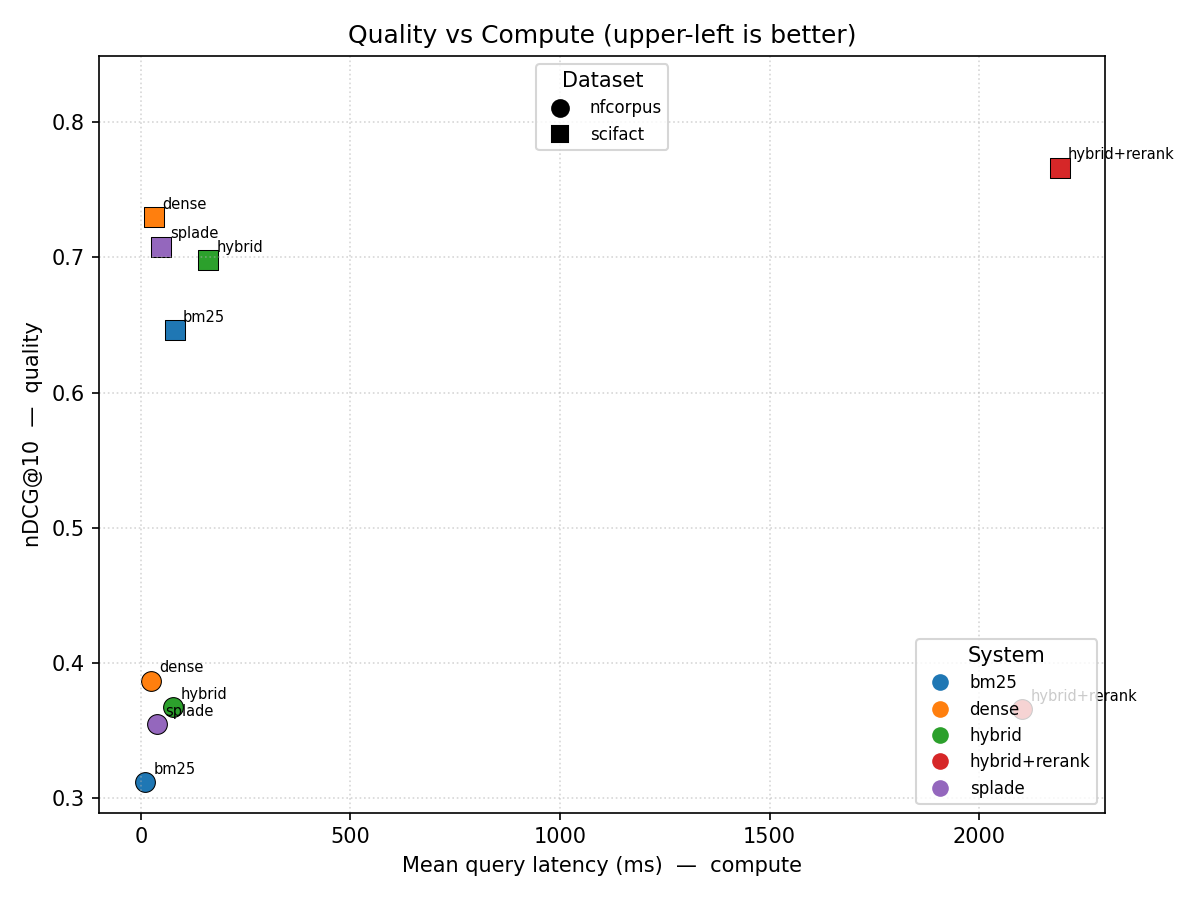
\includegraphics[width=0.8\linewidth]{pareto.png}}{%
    \fbox{\parbox{0.8\linewidth}{\centering\textit{eval/figures/pareto.png --- run the ablation + figures to populate}}}}
  \caption{Quality (nDCG@10) vs compute (mean query latency). Color = system,
           marker = dataset.}
  \label{fig:pareto}
\end{figure}

\begin{figure}[h]
  \centering
  \IfFileExists{../eval/figures/per_dataset_bars.png}{%
    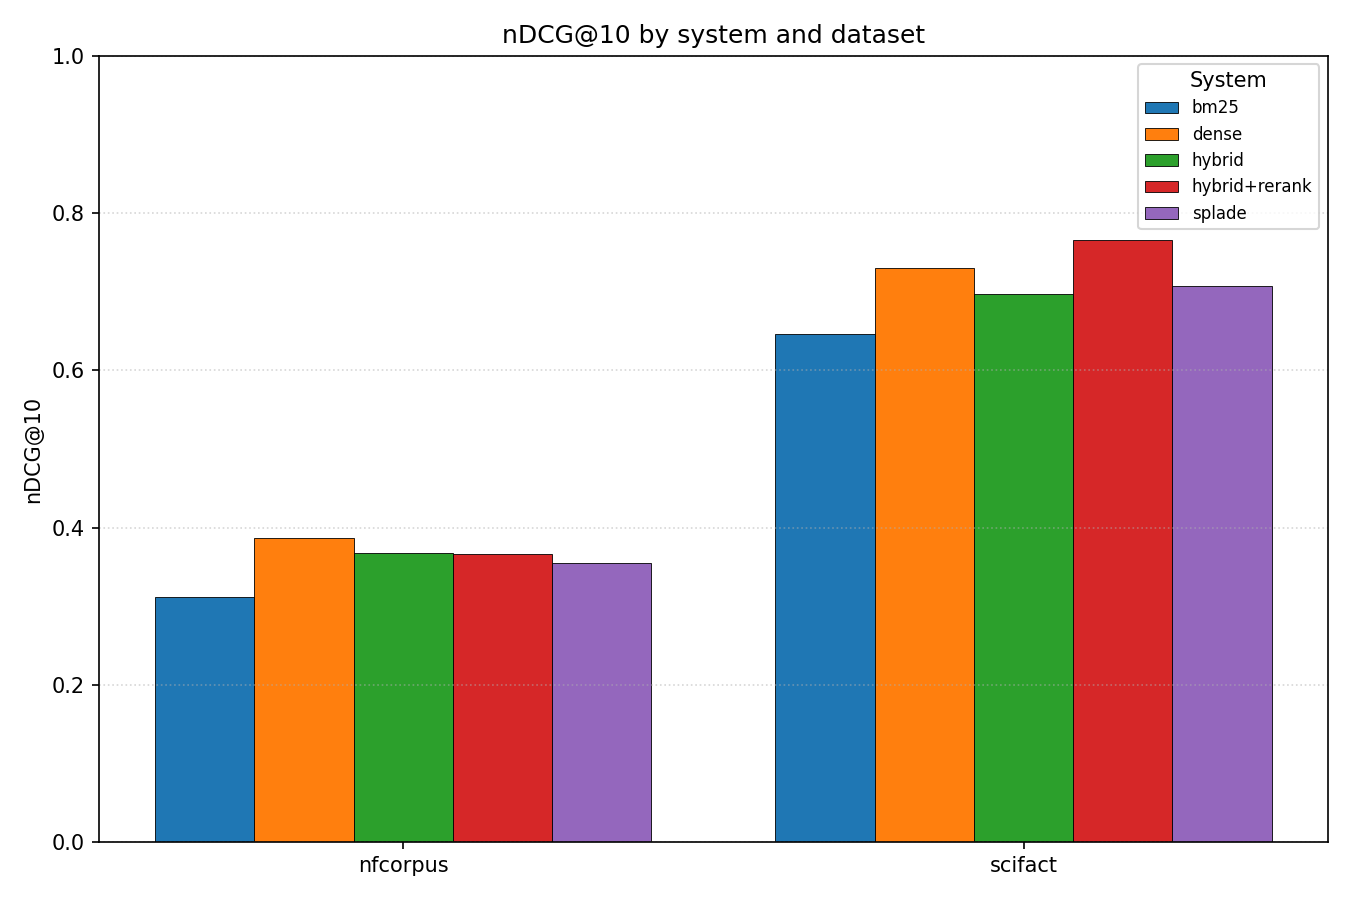
\includegraphics[width=0.8\linewidth]{per_dataset_bars.png}}{%
    \fbox{\parbox{0.8\linewidth}{\centering\textit{eval/figures/per\_dataset\_bars.png --- run the ablation + figures to populate}}}}
  \caption{nDCG@10 by system and dataset.}
  \label{fig:bars}
\end{figure}

\section{Discussion}
\label{sec:discussion}

\paragraph{A laptop-reproducibility hazard (the headline lesson).}
Our first set of runs reported an NFCorpus SPLADE nDCG@10 of 0.17 --- roughly half
the 0.35 reported for the same checkpoint
(\texttt{splade-cocondenser-ensembledistil}) in the literature. Because every
other baseline matched published values (dense 0.387, BM25 0.31), the anomaly was
isolated to SPLADE. The cause was neither the model nor the metric but the
hardware: on Apple Silicon (\texttt{mps}), \texttt{torch.max} along the sequence
axis returns incorrect results for \emph{short, lightly-padded} inputs. Short
SPLADE queries (e.g.\ ``Foods for Glaucoma'') were max-pooled into nonsense term
expansions (punctuation and stopword pieces) instead of their salient terms,
quietly destroying ranking on exactly the queries a sparse model should handle
well. The fix is one line --- pad every batch to a fixed length
(\texttt{padding="max\_length"}) rather than to the batch maximum --- after which
\texttt{mps} reproduces CPU bit-for-bit and SPLADE recovers to 0.355 on NFCorpus
and 0.708 on SciFact, both in line with published numbers. We surface this
explicitly because the field increasingly runs IR experiments on Apple-Silicon
laptops, where such silent numerical divergences are easy to mistake for a weak
model and bake into a leaderboard.

Beyond that, the ablation makes three things measurable rather than assumed.
First, the cosine-vs-L2 comparison (Table~\ref{tab:cosvl2}) is a correctness fix
whose \emph{empirical} impact depends on the embedder: \texttt{embeddinggemma-300m}
produces near-unit-norm vectors, so cosine and L2 rank almost identically here
(delta within noise). The fix is still the right default --- it guarantees the
intended geometry regardless of an embedder's norm distribution --- but we report
the near-zero delta honestly rather than claiming a win the data does not support.
Second, with all three retrievers now at full strength, the picture across
datasets is corpus-dependent: on SciFact dense leads the single retrievers (0.730)
with SPLADE close behind (0.708), while on the harder NFCorpus dense (0.387) edges
SPLADE (0.355) and BM25 (0.312). Equal-weight hybrid lands between its components
rather than strictly above them, so the value of fusion is conditional on
corpus-appropriate weights --- the case for the learned, query-adaptive routing in
the future-work roadmap. Third, the Pareto view (Figure~\ref{fig:pareto})
quantifies the reranker's bargain: cross-encoder reranking is the clearest win on
SciFact (hybrid+rerank 0.766, the best system there) but adds two orders of
magnitude more latency, so whether it pays off is itself corpus-dependent.

\section{Limitations and Future Work}
\label{sec:future}

This sprint is deliberately bounded. It evaluates two small datasets, not the
full BEIR-13 or LoTTE; it uses off-the-shelf models without fine-tuning; and the
fusion weights are swept rather than learned. The broader research roadmap, scoped
out here, comprises three directions: (i) a \emph{Query-Adaptive Retriever Router}
that predicts per-query which retrievers to fire and at what depth --- with the
three-retriever pool (BM25, dense, SPLADE) already in place, the open
question is whether such a router learns to invoke the more expensive retrievers
only when they pay off; (ii) \emph{Cascade Reranking with Confidence-Based
Early Exit}, which stops reranking once the top-$k$ order has stabilized; and
(iii) \emph{LLM-Distilled Domain Embeddings} trained on hard triplets where a
frontier model selects hard negatives from the real corpus. Each targets the
efficiency or domain-adaptation frontier that the present quality--compute analysis
only measures. Scaling to a 1M-document technical corpus (S2ORC + arXiv) is the
natural data axis for those contributions.

\section{Conclusion}
\label{sec:conclusion}

Beetle shows that a small hybrid search system becomes a credible research artifact
not by adding novelty but by being measured: fix the metric bug, include every
retriever in fusion, and report a reproducible quality--compute ablation on public
benchmarks. The result is a system whose every claim is backed by a versioned,
pinned, property-tested pipeline that runs on a laptop.

\bibliographystyle{plain}
\bibliography{references}

\end{document}
